% !TeX program = xelatex
% !TEX encoding = UTF-8 Unicode

\documentclass[9pt]{article}
\usepackage[paperheight=6cm,paperwidth=6cm]{geometry}
\usepackage{mfirstuc}
\usepackage{graphicx}
\usepackage{tikz}
\usepackage{float}
\usepackage{xcolor}
\usepackage{setspace}
\usepackage{kantlipsum}
\usepackage{tabularx}
\usepackage{array}
\newcommand{\PreserveBackslash}[1]{\let\temp=\\#1\let\\=\temp}
\newcolumntype{C}[1]{>{\PreserveBackslash\centering}p{#1}}
\newcolumntype{R}[1]{>{\PreserveBackslash\raggedleft}p{#1}}
\newcolumntype{L}[1]{>{\PreserveBackslash\raggedright}p{#1}}

\usepackage{fontspec}
% \usepackage[sfdefault,light]{roboto}  %% Option 'sfdefault' only if the base font of the document is to be sans serif
% \usepackage[T1]{fontenc}
% \setmainfont{Ubuntu}

\geometry{
	left=.2cm,
	right=.2cm,
	top=.7cm,
	bottom=0cm
}

\definecolor{maincolor}{HTML}{ffffff}
\definecolor{bgcolor}{HTML}{000080}

\newcommand{\nuovipositiviwrapper}[1]{{\selectfont\Huge\color{maincolor}\textbf{#1}}}
\newcommand{\rcolumn}[1]{\hspace{-.35cm}\textbf{#1}}
\newcommand{\lcolumn}[1]{\footnotesize#1}

\newcommand{\datawrapper}[1]{\scriptsize#1}

\input{numbers.txt}

\tikzset{zlevel/.style={%
	execute at begin scope={\pgfonlayer{#1}},
	execute at end scope={\endpgfonlayer}
}}

\begin{document}
		
	\pagestyle{empty}

	\tikz[remember picture,overlay, baseline=0.6ex]\path [fill=bgcolor] (-1cm,-.55cm) rectangle (7cm,2cm);

	\vspace{-1.5cm}
	
	\begin{center}
		\noindent\nuovipositiviwrapper{{\Large\raisebox{.6ex}{+}}\nuovipositivi\\\normalsize\indent~~nuovi contagi}
		\vfill
		
		\begin{tikzpicture}[remember picture,overlay]
			\node[
			opacity=.2,
			left=-200pt,
			] at (current page.south west)
			{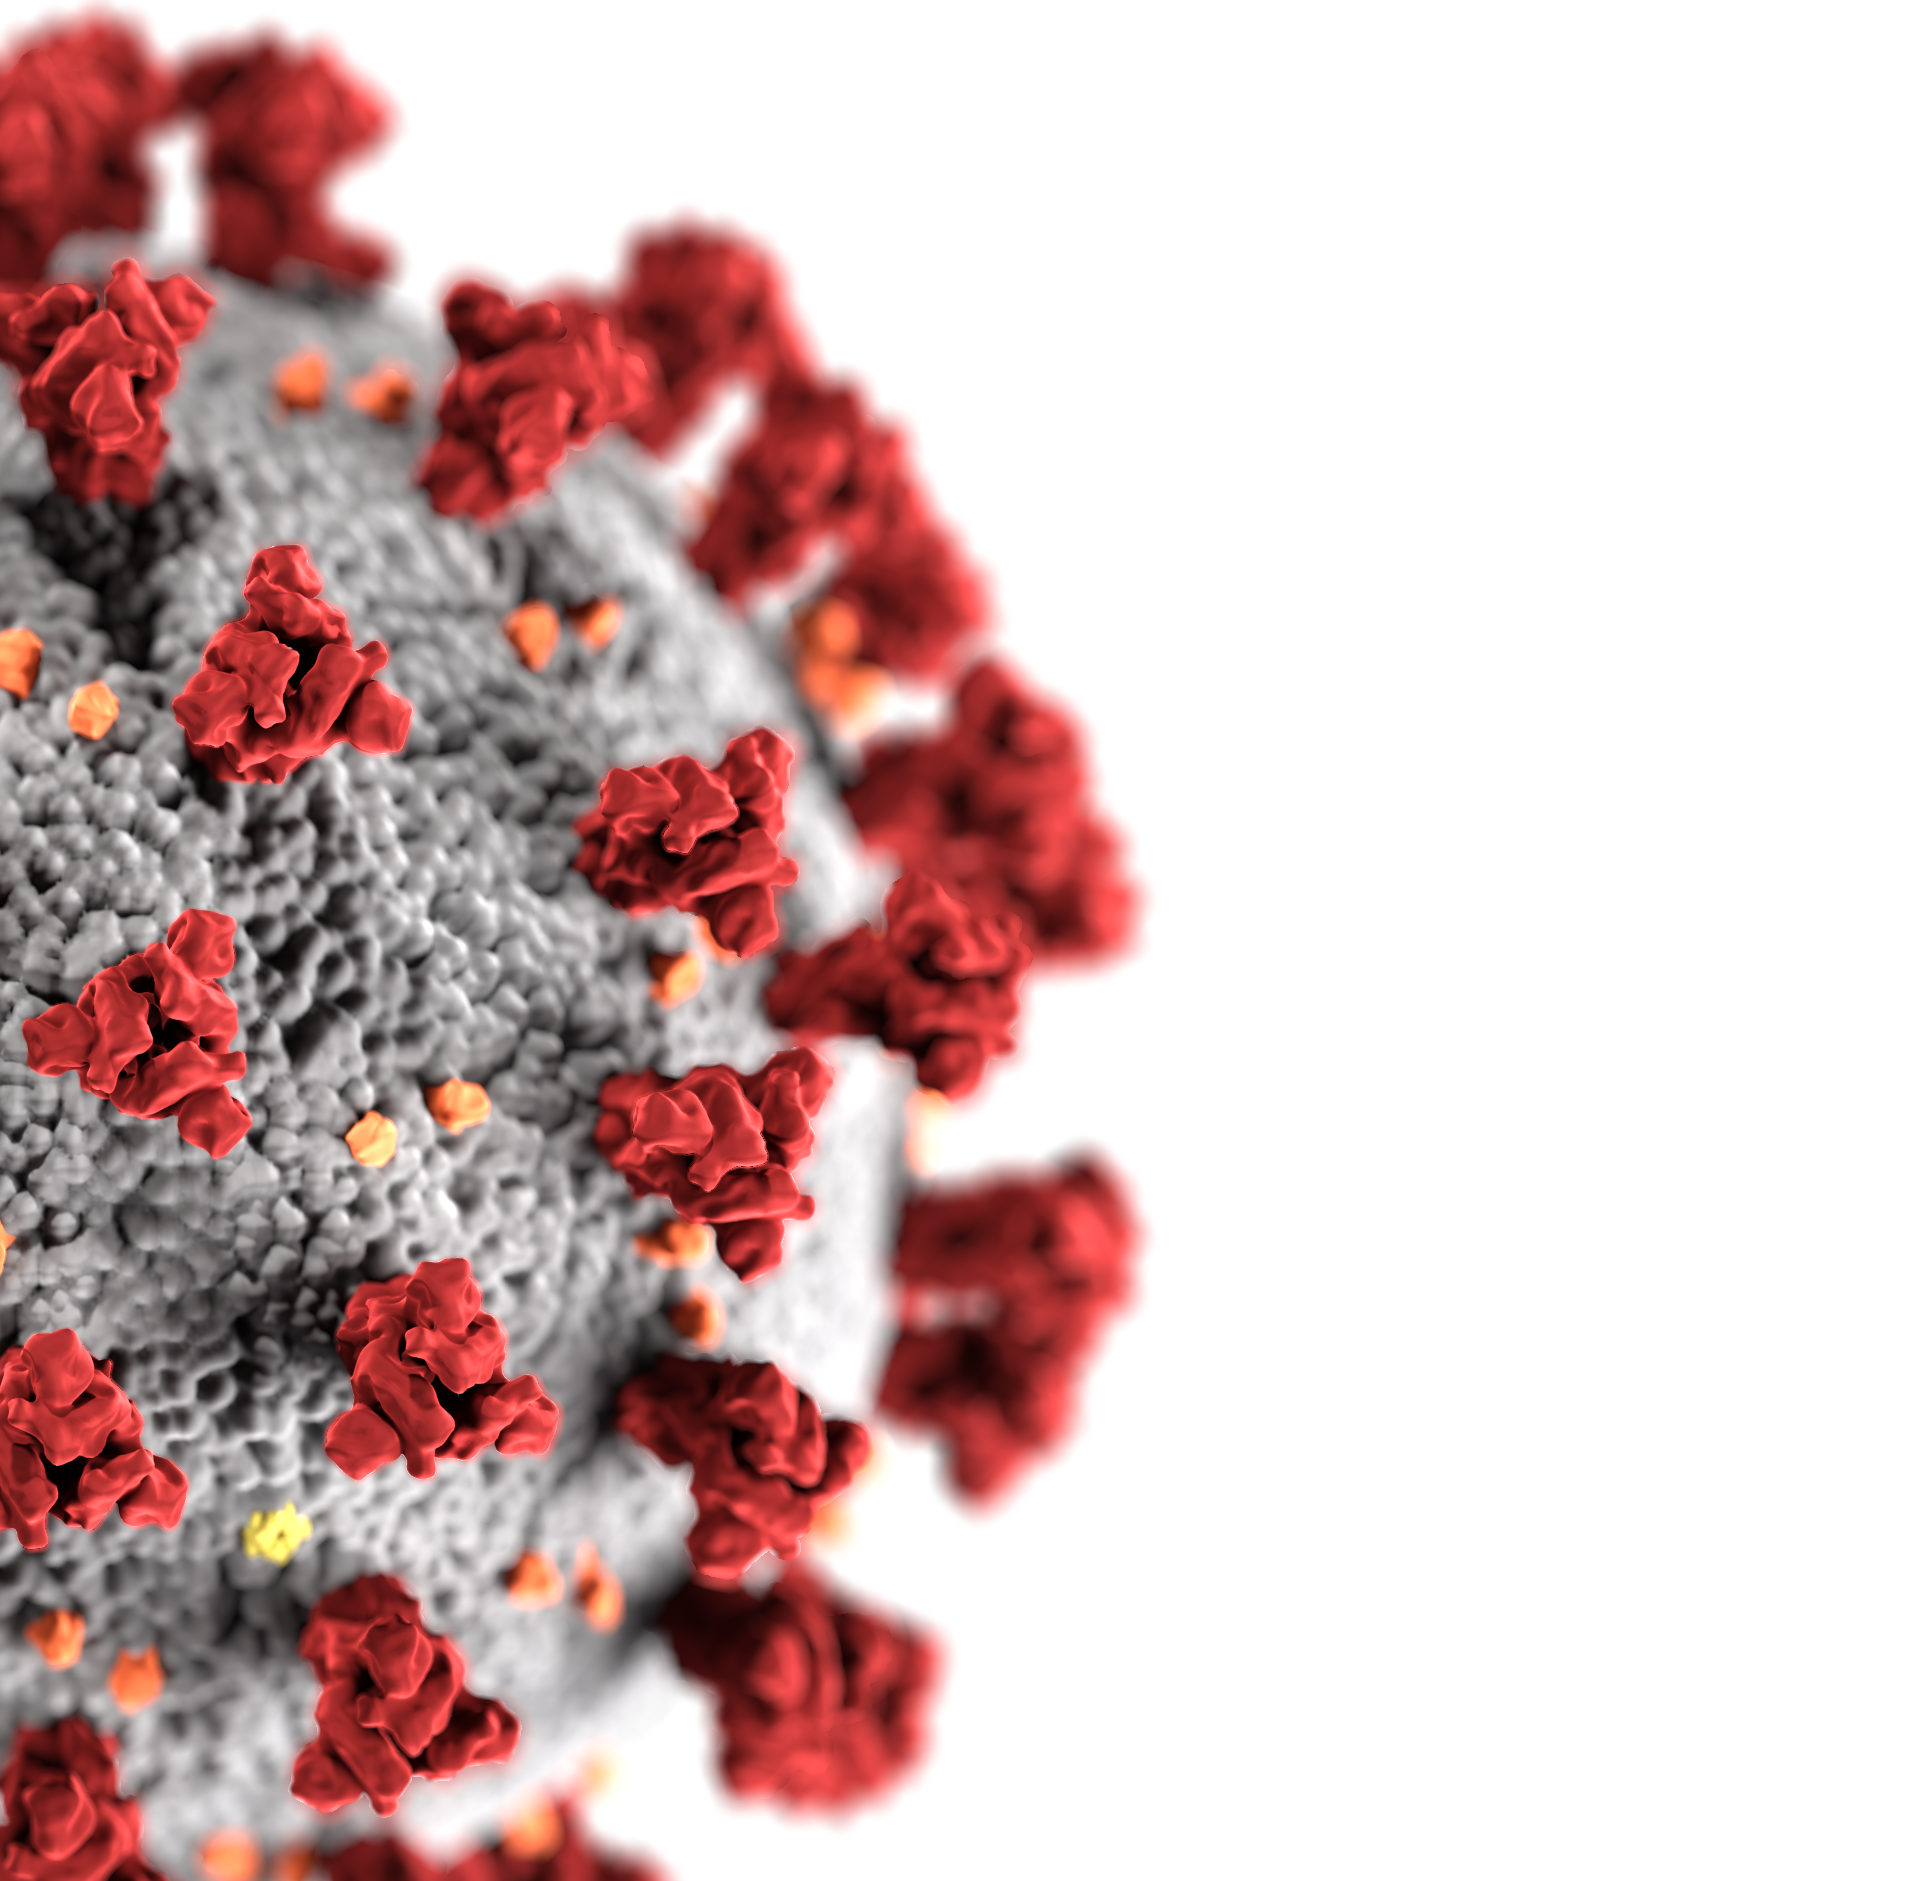
\includegraphics[height=7cm]{img/bkg_2}};
		\end{tikzpicture}
		
		\renewcommand{\arraystretch}{1.3}
		
		\begin{tabular}{L{3.2cm}R{1.2cm}}
			\lcolumn{Totali positivi}			& 		\rcolumn{\totalipositivi}			\\
			\lcolumn{Totale ospitalizzati}		& 		\rcolumn{\totaleospitalizzati}		\\
			
		\end{tabular}
		\renewcommand{\arraystretch}{.5}
		\begin{tabular}{L{3.2cm}R{1.2cm}}
			\lcolumn{\tiny Di cui ricoverati con sintomi}
			&
			\rcolumn{\footnotesize\ricoveratisintomi}\\
			\lcolumn{\tiny Di cui in terapia intensiva}
			& 
			\rcolumn{\footnotesize\terapiaintensiva}\\
		\end{tabular}
		\renewcommand{\arraystretch}{1.3}
		\begin{tabular}{L{3.2cm}R{1.2cm}}
			\lcolumn{Isolamento domiciliare}			& 		\rcolumn{\isolamento}			\\
			\lcolumn{Deceduti}					& 		\rcolumn{\deceduti}					\\
		\end{tabular}
		\vfill
		\begin{tabular}{m{3.2cm}m{1.2cm}}
			\capitalisewords{\zona}\newline\datawrapper{\data}
			&
			\PreserveBackslash\raggedleft\includegraphics[width=1cm,height=.75cm,interpolate,keepaspectratio]{img/\zona}
		\end{tabular}
	
		\vfill
	
	\end{center}

\end{document}